\documentclass[acmlarge, screen, nonacm]{acmart}
\usepackage[utf8]{inputenc}
\usepackage{CJKutf8}
\usepackage{graphicx}
\usepackage{pgf}
\usepackage{multicol}
\usepackage{setspace}
\usepackage{listings}
\usepackage{hyperref}
\usepackage{float}
\usepackage{placeins}
\graphicspath{ {./images/} }
\usepackage{tikz}
\usepackage{verbatim}
\usepackage{cleveref}
\usepackage{datetime}
\usepackage{longtable}

\crefname{figure}{Figure}{Figures}
\usetikzlibrary{trees}
\usetikzlibrary{arrows}

\definecolor{codegreen}{rgb}{0,0.6,0}
\definecolor{codegray}{rgb}{0.5,0.5,0.5}
\definecolor{codepurple}{rgb}{0.58,0,0.82}
\definecolor{backcolour}{rgb}{0.95,0.95,0.92}
\definecolor{OrangeRed}{rgb}{1,0.27,0}
\definecolor{ForestGreen}{rgb}{0.1334,0.545,0.1334}
\definecolor{NavyBlue}{rgb}{0,0.502,0}
\definecolor{BurntOrange}{rgb}{0.8,0.3334,0.1334}
\definecolor{selectColor}{rgb}{0.686,1,0.592}

\newcommand\YAMLcolonstyle{\color{black}\mdseries}
\newcommand\YAMLkeystyle{\color{BurntOrange}\bfseries}
\newcommand\YAMLvaluestyle{\color{black}\mdseries}

\lstdefinelanguage{yaml}
{
  keywords={true,false,null,y,n},
  keywordstyle=\color{darkgray}\bfseries,
  basicstyle=\YAMLkeystyle,
  sensitive=false,
  comment=[l]{\#},
  morecomment=[s]{/*}{*/},
  commentstyle=\color{ForestGreen}\ttfamily,
  stringstyle=\YAMLvaluestyle\ttfamily,
  moredelim=[l][\color{orange}]{\&},
  moredelim=[l][\color{magenta}]{*},
  moredelim=**[il][\YAMLcolonstyle{:}\YAMLvaluestyle]{:},
  morestring=[b]',
  morestring=[b]",
  literate =    {---}{{\ProcessThreeDashes}}3
                {>}{{\textcolor{red}\textgreater}}1
                {|}{{\textcolor{red}\textbar}}1
                {\ -\ }{{\mdseries\ -\ }}3,
}

\lstdefinestyle{mystyle}{
	backgroundcolor=\color{backcolour},
	commentstyle=\color{codegreen},
	keywordstyle=\color{magenta},
	numberstyle=\tiny\color{codegray},
	stringstyle=\color{codepurple},
	basicstyle=\sffamily\footnotesize,
	breakatwhitespace=false,
	breaklines=true,
	captionpos=b,
	keepspaces=true,
	numbers=left,
	numbersep=5pt,
	showspaces=false,
	showstringspaces=false,
	showtabs=false,
	tabsize=2
}

\lstdefinelanguage{Kotlin}{
  comment=[l]{//},
  commentstyle={\color{gray}\ttfamily},
  emph={delegate, filter, first, firstOrNull, forEach, lazy, map, mapNotNull, println, return@},
  emphstyle={\color{OrangeRed}},
  identifierstyle=\color{black},
  keywords={abstract, actual, as, as?, break, by, class, companion, continue, data, do, dynamic, else, enum, expect, false, final, for, fun, get, if, import, in, interface, internal, is, object, override, package, private, public, return, set, super, suspend, throw, true, try, typealias, val, var, vararg, when, where, while},
  keywordstyle={\color{NavyBlue}\bfseries},
  morecomment=[s]{/*}{*/},
  morestring=[b]",
  morestring=[s]{"""*}{*"""},
  ndkeywords={@Deprecated, @JvmField, @JvmName, @JvmOverloads, @JvmStatic, @JvmSynthetic, Array, Byte, Double, Float, this, null, Int, Integer, Iterable, Long, Runnable, Short, String, Boolean},
  ndkeywordstyle={\color{BurntOrange}\bfseries},
  sensitive=true,
  stringstyle={\color{ForestGreen}\ttfamily},
}

\lstset{style=mystyle}
\settopmatter{printacmref=false}
\settopmatter{printfolios=true}
\setcopyright{none}
\makeatletter
\let\@authorsaddresses\@empty

\makeatletter
\let\newdate\@date

\settopmatter{printacmref=false}
\setcopyright{none}
\renewcommand\footnotetextcopyrightpermission[1]{}
\pagestyle{plain}

\begin{document}
\begin{CJK*}{UTF8}{gbsn}

\title[]{
  
\includegraphics[width = 150pt, height = 150]{pictures/logo.png}\\
  DiKTat - Kotlin linter
}

\author{Andrey Kuleshov}
\email{andrewkuleshov7@gmail.com}
\affiliation{
\institution{Lomonosov Moscow State University}
\country{Russia}
}
\author{Petr Trifanov}
\email{peter.trifanov@mail.ru}
\affiliation{
\institution{Lomonosov Moscow State University}
\country{Russia}
}
\author{Denis Kumar}
\email{qbextted0@gmail.com}
\affiliation{
\institution{Higher School of Economics}
\country{Russia}
}
\author{Alexander Tsay}
\email{aktsay6@gmail.com}
\affiliation{
\institution{Higher School of Economics}
\country{Russia}
}

\renewcommand{\shortauthors}{}

\maketitle

\section{Introduction}
\label{sec:intro}
It is necessary to conform to a specific style of code during software development, otherwise it will lead to difficulties in reading and writing the program. The static analyzer, in turn, has methods for finding and correcting style errors. There are both open source\footnote{PMD: \url{http://pmd.sourceforge.net/}, Rubocop: \url{https://github.com/rubocop-hq/rubocop},
PHPCS: \url{https://github.com/squizlabs/PHP_CodeSniffer}
FindSecBugs: \url{https://find-sec-bugs.github.io/}, ESLint: \url{https://eslint.org/}, Checkstyle: \url{https://checkstyle.sourceforge.io/}.}
(PMD, Rubocop, PHPCS, FindSecBugs, ESLint, Checkstyle, to name a few) and commercial\footnote{IBM Security AppScan: \url{https://www.hcltechsw.com/wps/portal/products/appscan},
PVS-Studio: \url{https://www.viva64.com/en/pvs-studio/},
SonarQube: \url{https://www.sonarqube.org/},
Parasoft: \url{https://www.parasoft.com/}}
(IBM Security AppScan, PVS-Studio, SonarQube, Parasoft) static analyzers
on the market.

Of the tasks solved by static code analysis programs, two main ones can be distinguished: identifying errors
in programs and recommending code formatting. That is, the analyzer allows you to check whether the source
code complies with the accepted coding standard. Also, a static analyzer can be used to determine the
maintainability of a code, which is how easy it is to analyze, modify and adapt a given software.

Functional quality aspects are typically quite susceptible to formal definition
and quantification.
% (\todo: examples!!).
Functional quality is also an essential
requirement in any domain of software development. On the other hand,
maintainability is a lot less straightforward to formally specify or quantify.
%\todo: refs.
Also, in certain applications it appears less important than
functional correctness, although in business domain it is recognized as an
essential property.
% (\todo: ref).
As a result, there are currently a lot more
research and practical tools addressing functional quality aspects of code than
maintainability \citep{Overview_Static_Code_Analysis_in_Software_Development}.
Another aspect of static analysis tools that may have hindered their application
to maintainability, is that they are predominantly rule-based. Since there has
not yet been a consensus on how to formalize maintainability, it is challenging
to devise a set of formal rules to detect it.

We designed our new tool Aibolit to help developers identify patterns in their
code  that may cause maintainability issues. It is a next generation static
analysis tool that uses a machine learning (ML) model as an underlying quality
prediction mechanism. From the perspective of ML, our product is a recommender
system. For a given class file, it gives suggestions to the developer to alter
their code. The recommendations come in the form of \textit{code patterns} that
are detected in the code and advised to be removed.

Our choice to design Aibolit as a ML-based system alleviates some important
shortcomings of rule-based static analyzers. By design, ML algorithms capture
statistical relations in the external world (data). Therefore, they can be a
good way to model imprecisely and subjectively defined properties of code, such
as its maintainability. Moreover, rule-based system are known to not scale well
to the diversity of empirically observed cases, and they tend to get very hard
to extend and maintain \citep{LenatFeigenbaum1987}. The ML
approach does not require
manual system adaptation as new observations or new features (patterns) come
along. In fact, Aibolit provides an easy way for developers to integrate a code
pattern of their liking into the recommender system and to analyze the pattern`s
impact on code quality.

\section{Definition}
\label{sec:definition}
Before we will move one, it is necessary to define some terms so that the reader correctly understands the context of what was written. 
The first and basic concept that should be introduced is \textbf{Rule} (marked with $R_i$). Rule in diKTat - is the logic described in a special class named with \texttt{"Rule"} suffix, which checks that a code is compliant with a certain paragraph of code-style. From the basics of maths you should know that the set - is a well-defined collection of distinct objects, considered as an object in its own right. So we can define a \textbf{Ruleset} - a set of such code analysis Rules. We will mark any of such set of Rules with $R$.

\textbf{Inspection} - is the part of any Rule. It is an algorithm that can detect (marked with $W_i$) or fix (marked with $F_i$) invalid code. It is very important to understand that $Rule \neq Inspection$. We will use $I_i$ notation to mark each separate inspection. So it is obvious that: $I_{ij} = \bigcup\limits_{i, j} W_{i} \cup F_{j}$, where $i, j \in \mathbb {N}$. Using the same logic we can say that $R = \bigcup\limits_{i} R_i$ where $R_i = \bigcup\limits_{i} I_i$.

\textbf{Abstract syntax tree (AST)} is a tree representation of the abstract syntactic structure of source code written in a programming language (Kotlin in our case). Each node of the tree denotes a construct occurring in the source code. \textbf{CI/CD} - continuous integration (CI) and continuous delivery (CD) is a methodology that allows application development teams to make changes to code more frequently and reliably \cite{ref:cicd}. \textbf{KDoc} - is the language used to document Kotlin code (the equivalent of Java's JavaDoc).

\section{Kotlin}
\label{sec:kotlin}
\par Kotlin is a cross-platform, statically typed, general-purpose programming language with type inference. Kotlin is designed to interoperate fully with Java, and the JVM version of Kotlin's standard library depends on the Java Class Library, but type inference allows its syntax to be more concise. Kotlin mainly targets the JVM, but also compiles to JavaScript (e.g. for frontend web applications using React) or native code (via LLVM), e.g. for native iOS apps sharing business logic with Android apps. % wikipedia

\par Kotlin has quickly skyrocketed in popularity. It's used by companies like Google, Square, Pinterest, Pivotal, Netflix and Atlassian. It's the fastest-growing programming language, according to GitHub, growing over 2,5 times in the past year. It was voted one of the five most loved languages, according to Stack Overflow. There are even meetups focused on Kotlin. 
% https://www.businessinsider.com/kotlin-programming-language-explained-popularity-2019-5#:~:text=Kotlin%20has%20quickly%20skyrocketed%20in,times%20in%20the%20past%20year.
\par Kotlin is used in a lot of ways. For example it can be used for backend development using ktor framework (developed by JetBrains), and spring framework also has first-party support for kotlin (Spring is one of the most popular framework on Java for Web development). Kotlin/JS provides the ability to transpile your Kotlin code to JavaScript, as well as providing JS variant of kotlin standard library and interopability with existing JS dependencies, both for Node.js and browser. There are numerous ways that Kotlin/JS can be used. For instance, you can write frontend web applications using Kotlin/JS,
write server-side and serverless applications using Kotlin/JS, create libraries for use with JavaScript and TypeScript. Support for multiplatform programming is one of Kotlin’s key benefits. It reduces time spent writing and maintaining the same code for different platforms while retaining the flexibility and benefits of native programming. 

\par Asynchronous or non-blocking programming is the new reality. Whether we're creating server-side, desktop or mobile applications, it's important that we provide an experience that is not only fluid from the user's perspective, but scalable when needed.
There are many approaches to this problem, and Kotlin takes a very flexible one by providing Coroutine support as a first-party library kotlinx.coroutines with a kotlin compiler plugin and delegating most of the functionality to libraries, much in line with Kotlin's philosophy.
As a bonus, coroutines not only open the doors to asynchronous programming, but also provide a wealth of other possibilities such as concurrency, actors, etc.

A coroutine is a concurrency design pattern that you can use on Android to simplify code that executes asynchronously. Coroutines(in a form of kotlinx.coroutines library and kotlin compiler plugin) were added to Kotlin in version 1.3 and are based on established concepts from other languages.

On Android, coroutines help to manage long-running tasks that might otherwise block the main thread and cause your app to become unresponsive. Over 50\% of professional developers who use coroutines have reported seeing increased productivity. Coroutines enable you to write cleaner and more concise app code.

The state of Kotlin in 2020 (according to the latest Kotlin Census and statistical data)
\begin{itemize}
    \item 4,7 million users
    \item 65\% of users use Kotlin in production
    \item For 56\% of users, Kotlin is their primary language, which means the main or only
    one they use at work
    \item 100+ people are on the Kotlin development team at JetBrains
    \item 350+ independent contributors develop the language and its ecosystem outside
    of JetBrains
\end{itemize}

% https://techcrunch.com/2019/05/07/kotlin-is-now-googles-preferred-language-for-android-app-development/
Kotlin is widely used among Android developers, including open source OS, like HarmonyOS, that are compatible with Android. In 2019 Google announced that the Kotlin programming language is now its preferred language for Android app developers. In the same year Stack Overflow stated that Kotlin is fourth most loved language in community. Nowadays there are over 60\% of android developers who use Kotlin as their main language. 
\par Kotlin's popularity can be explained by the rising number of Android users (last year, 124.4m in the USA) and, thus, Android-based devices. 80\% of Kotlin programmers use the language to build Android apps, 31\% for back-end applications, 30\% for SDK/libraries.
Kotlin is also interoperable with Java, which allows developers to use all existing Android libraries in a Kotlin app. Kotlin is in the top of PYPL rating.
\newline
\includegraphics[scale =0.65]{pictures/kotlinRating.png}
\newline
\par Overall, Kotlin is a modern language that gain it's popularity incredibly fast. It is mostly used by Android developers, but other "branches of programming" are gaining popularity as well, for example spring framework(the most popular Java framework) is supporting Kotlin. It supports both OO (object-oriented) and FP (function-oriented) programming paradigms. Since release 1.4 Kotlin claims to bring major updated every 6 month.

\section{diKTat}
\label{sec:diKTat}
\subsection{What is diKTat?}
DiKTat \footnote{\url{https://github.com/cqfn/diKTat}} - is a formal strict code-style for Kotlin language and a linter with a set of rules that implement this code-style. Basically, it is a collection of Kotlin code style rules implemented as AST visitors on top of KTlint framework \footnote{\url{https://github.com/pinterest/ktlint}}. Diktat detects and automatically fixes code style errors and code smells based the configuration of rules. DiKTat is a highly configurable framework, that can be extended further by adding custom rules. It can be run as command line application or with maven or gradle plugins. In this paper, we will explain how diKTat works, describe it's advantages and disadvantages and compare it with other static analyzers for Kotlin. The main idea is to use diktat in your CI/CD pipeline.

\subsection{Why diKTat?}
So why did we decide to create diKTat? We looked at similar existing projects and realized that their functionality does not give us a chance to implement our own configurable code style. Most of rules that we wanted to implement were missing in other analyzers. Mostly all of those analyzers had hardcoded logic and prohibited configuration. That’s why we decided that we need to create convenient and user friendly tool for developers that can be easily configured. Why is it easy-to-use?

First of all, diKTat has its own highly configurable Ruleset $R_{diktat}$ that contains unique Inspections that are missing in other Kotlin static analyzers. You just need to set your own options that fit your project the most. In case you don't want to do this - you can use the default configuration, but some of complex inspections will be disabled. Basically, Ruleset is an \texttt{yml} file with a description of each rule. 

Secondly, diKTat has it's own plugins and can be run via Maven, Gradle and command line. Developer can use build automation system that he prefers.

Finally, with diKTat developer can disable each inspection from the code using special annotations on the line where he wants to suppress an Inspection.

\section{Comparative analysis}
\label{sec:compare}
\subsection{About ktlint}
Ktlint is a popular an anti-bikeshedding Kotlin linter with a built-in formatter created by Pinterest\footnote{\url{https://github.com/pinterest/}}. It tries to reflect official code style from \texttt{kotlinlang.org} and Android Kotlin Style Guide and then automatically apply these rules to your codebase. Ktlint can check and automatically fix code. It claims to be simple and easy to use. As it is focused more on checking code-style and code-smell related issues, ktlint inspections work with Abstract Syntax Tree generated by Kotlin parser. Ktlint framework has some basic utilities to make the work with Kotlin AST easier, but anyway all inspections work with original ASTNode provided by Kotlin parser.

Ktlint has been developed since 2016 and since then it has 3.8k stars, 309 forks and 390 closed PRs (2020). It looks to be the most popular and mature linter in the Kotlin community right now with approximately 15k lines of code written.

Ktlint has its own set of rules, which are divided on standard and experimental rules. But unfortunately the number of fixers and checkers in the standard ruleset is very few (~20 rules) and inspections are trivial.

Ktlint can be used as a plugin for Maven, Gradle or command line app. \texttt{.editorconfig} file should be modified to configure rules. This is the - only configuration that ktlint provides and it contains just simple configuration like the number of spaces in indents. Actually user even can’t configure specific rules (for example to disable or suppress any of them), instead you can provide some common settings like the number of spaces for indenting. In other words, ktlint has a "fixed hardcoded” code-style that is not very configurable.

If you want to implement your own rules you need to create a your own Ruleset. Ktlint is very user-friendly for creation of custom Rulesets. In this case ktlint will parse the code using a Kotlin parser and will trigger your inspection (as visitor) for each node of AST. Ktlint uses javas \texttt{ServiceLoader} to discover all available Rulesets. \texttt{ServiceLoader} is used to inject your own implementation of rules for the static analysis. In this case ktlint becomes both a third-party dependency and a framework. Basically you should provide implementation of \texttt{RuleSetProvider} interface.

Ktlint refers to article on Medium\footnote{\url{https://medium.com/mydevnotes/ktlint-improve-your-kotlin-code-quality-with-lint-checks-13a4456c4600}} on how to create a custom Ruleset and a Rule.

A lot of projects uses ktlint as their code formatting tool. For example, OmiseGo \footnote{\url{https://github.com/omgnetwork/android-sdk}} (currently rebranding to OMG Network) - is a quite popular cryptocurrency.

To summarize: Ktlint is very mature and useful as a framework for creating your own checker\&fixer of Kotlin code and doing AST-analysis. It can be very useful if you need only simple inspections that check (and fix) code-style issues (like indents).

\begin{figure}[H]
    \centering
    \includegraphics[scale = 0.6]{pictures/ktlint.png}
    \caption{Ktlint Code Frequency}
    \label{fig:png_ktlint}
\end{figure}

\subsection{About detekt}
Detekt \footnote{\url{https://github.com/detekt/detekt}} is a static code analysis tool. It operates on an abstract syntax tree (AST) and meta-information provided by Kotlin compiler. On the top of that info, it does a complex analysis of the code. However, this project is more focused on checking the code rather than fixing. Similarly, to ktlint, it has its own rules and inspections. Detekt uses wrapped ktlint to redefine RuleSet of ktlint as it’s formatting rules.

Detekt supports detection of code smells, bugs searching and code-style checking. It has a highly configurable rule sets (can even make suppression of issues from the code). And the number of checkers is large: it has more than 100 inspections. Detekt has IntelliJ integration, third-party integrations for Maven, Bazel and Github actions and a mechanism for suppression of their warnings with @Suppress annotation from the code. It is being developed since 2016 and today it has 3.2k stars, 411 forks and 1850 closed PRs. It has about 45k lines of code. And its codebase is the biggest comparing to other analyzers.
Detekt is used in such projects as fountain \footnote{\url{https://github.com/xmartlabs/fountain}} or Kaspresso   \footnote{\url{https://github.com/KasperskyLab/Kaspresso}}.

To summarize: Detekt is very useful as a Kotlin static analyser for CI/CD. It tries to find bugs in the code and is focused more on checking of the code. Detekt has 100+ rules which check the code.

\begin{figure}[H]
    \centering
    \includegraphics[scale = 0.6]{pictures/detekt.png}
    \caption{Detekt Code Frequency}
    \label{fig:png_detekt}
\end{figure}

\subsection{About ktfmt}
Ktfmt formats is a program that formats Kotlin code, based on google-java-format. Its development started in Facebook at the end of 2019. It can be added to client’s project through a Maven dependency, Gradle dependency, IntelliJ plugin or run through a command line. Ktfmt is not a configurable application, so to change any rule logic you need to download the project and redefine some constants. Ktfmt has 214 stars, 16 forks, 20 closed PRs and around 7500 lines of code.

To summarize: no one knows why Facebook has invested their money in this tool. Nothing new was introduced. If they really needed to have new rules - they could create their own Ruleset for ktlint or detekt.

\begin{figure}[H]
    \centering
    \includegraphics[scale = 0.6]{pictures/ktfmt.png}
    \caption{Ktfmt Code Frequency}
    \label{fig:png_ktfmt}
\end{figure}

\subsection{About diKTat}
Diktat is a static code analysis tool as well as ktlint and detect. But diktat is not only a tool, but also a coding convention that describes in details all the rules that you should follow when writing a code on Kotlin. Its development has started in 2020 and at the time of writing this article diKTat has 168 stars and 13 forks. DiKTat operates on AST provided by kotlin compiler. So why diKTat is better?

First of all, it supports much more rules than ktlint. Its ruleset includes more than 100 rules, that can both check and fix your code.

Secondly, diKTat is configurable. A lot of rules have their own settings, and all of them can be easily understood. For example, you can choose whether you need a copyright, choose a length of line or you can configure your indents.

Third, diKTat is very easy to configure. You don’t need to spend hours only to understand what each rule does. Diktat’s ruleset is a \texttt{.yml} file, where each rule is commented out with the description. Also you can suppress error on the particular lines of code using \texttt{@Suppress} annotation in your code.

DiKTat can be used as a CI/CD tool in order to avoid merging errors in the code. Overall it can find code smells and code style issues. Also it can find pretty not obvious bugs by complex AST analysis. Diktat works with maven, gradle and as command-line application powered by ktlint.

To summarize: diktat contains a strict coding convention that was not yet introduced by other linters. It works both as a checker and as a fixer. Diktat has much more inspections (100+) and is very configurable (each inspection can be disabled/configured separately), so you can configure it for your particular project.

\begin{figure}[H]
    \centering
    \includegraphics[scale = 0.6]{pictures/diktat.png}
    \caption{DiKTat Code Frequency}
    \label{fig:png_diktat}
\end{figure}

\subsection{A few words about Jetbrains}
Jetbrains invented  Kotlin and created one of the best IDEs for Java and Kotlin called IntelliJ. This IDE supports a built-in linter. However, it is not a well-configurable tool, you are not able to specify your own coding convention and it is not useful for CI/CD as it is highly coupled with UI. Unfortunately such static analysis is not so effective as it cannot prevent merging of the code with bugs into the repository. As experience shows - many developers simply ignore those static analysis errors until they are blocked from merging their pull requests. So it is not so suitable for CI/CD, but very good for finding and fixing issues inside your IDE.

\subsection{Summary}
To sum up, four linters, excepting diKTat, were mentioned above and each of them has it's own strengths and weaknesses. Diktat, in its turn, is uniting its strengths and providing new features in code linting and fixing tools.
\begin{center}
\begin{tabular}{ |p{3cm}|p{2.5cm}|p{2.5cm}|p{2.5cm}|p{2.5cm}| }
\hline
\multicolumn{5}{|c|}{\textbf{Comparing table}} \\
\hline
& diKTat& ktlint &detekt & ktfmt \\
\hline
starting year & 2020 & 2016 & 2016 & 2019 \\
stars & 168 & 3.2k & 3.8k & 214\\ 
forks & 13 & 299 & 411 & 16\\
closed PRs & 321 & 390 & 1850 & 20 \\
lines of code & 32k & 15k & 45k & 7,5k\\
number of rules & $>$100 & $\approx$ 20 & $>$100 & $\approx$ 10 \\
is configurable & yes & no & yes/no & no \\
maven/gradle plugin & both & both & gradle only & no \\
web version & yes & yes & no & no \\
\hline

\hline
\end{tabular}
\end{center}

\section{How does diktat work}
\label{sec:work}
Diktat does AST-analysis. This means that for internal representation (IR) it uses Abstract Syntax Tree that was created from the parsed code by the kotlin-compiler.  This chapter describes how diktat works

\subsection{ktlint}
\par
To quickly and efficiently analyze the program code, you first need to transform it into a convenient data structure. This is exactly what ktlint does - it parses plain text code into an abstract syntax tree. In ktlint, this happens in the \textsl{prepareCodeForLinting}\footnote{\url{https://github.com/pinterest/ktlint/blob/master/ktlint-core/src/main/kotlin/com/pinterest/ktlint/core/KtLint.kt}} method. This method uses Kotlin libraries to create a root node of type FILE.

\begin{figure}[H]
  \centering
  \includegraphics[scale=0.5]{wp/pictures/fileNode.PNG}
  \caption{Example of root Node}   
\end{figure} 

If there are error elements inside the constructed tree, then the corresponding error is displayed. Further, for each rule in the ruleset, the \textsl{visit} method is called to which the root node itself and its “children” are sequentially passed.
At startup, you can pass flags to ktlint - one of them is "-F". This flag means that the rule will not only report an error, but try to fix it.

\subsection{diKTat}
\par
Another feature of ktlint is that at startup you can transfer a JAR file with additional ruleset(s), and then all nodes will be passed to these rules. This is diKTat! DiKTat is a set of easily configurable rules for static code analysis. 
The set of all rules is described in the \textsl{DiktatRuleSetProvider}\footnote{\url{https://github.com/cqfn/diKTat/blob/master/diktat-rules/src/main/kotlin/org/cqfn/diktat/ruleset/rules/DiktatRuleSetProvider.kt}} class. This class overrides the \textsl{get()} method of the \textsl{RuleSetProvider}\footnote{\url{https://github.com/pinterest/ktlint/blob/master/ktlint-core/src/main/kotlin/com/pinterest/ktlint/core/RuleSetProvider.kt}} interface, which returns a set of rules to be "traversed". But before returning this set, the configuration file, in which the user has independently configured all the rules, is read. If there is no configuration file, then a warning will be displayed and the rules will be triggered in according with the default configuration file. 
Each rule must implement the \textsl{visit} method of the abstract Rule class, which describes the logic of the rule.

\begin{figure}[H]
  \centering
  \includegraphics[scale=0.5]{wp/pictures/ruleExample.PNG}
  \caption{Example of rule}   
\end{figure} 

The example above describes the rule in which you cannot write more than two statements on one line. The list of configurations is passed to the parameter of this rule so that the error is displayed only when the rule is enabled (further it will be described how to enable and disable the rule). The class fields and the \textsl{visit} method are described below. The first parameter in method is ASTNode - the node that we got in the parsing in ktlint. Then a check occurs: if the code contains a line in which more than one statement per line and this rule is enabled, then the rule will be executed and, depending on the mode in which the user started ktlint, the rule will either simply report an error or fix it. In our case, when an error is found, the method is called to report and fix the error - \textsl{warnAndFix()}.

\subsection{Examples of unique inspections}
\par


\section{Killer-Features}
\label{sec:feature}
\par As described above, diKTat is configurable and user-friendly. But these are not all of it's advantages and features. Below we will present and describe unusual and important killer-features of diKTat.

\subsection{Configuration file}
\par
It's worth starting with the configuration file. This is a file in which the user can manually turn rules on and off or configure the rules settings. Below is one of the rules in the configuration file.
\\
\begin{lstlisting}[ caption={Part of configuration file.},
label={lst:example1}, language=yaml]
- name: DIKTAT_COMMON
  configuration:
    # put your package name here - it will be autofixed and checked
    domainName: your.name.here
- name: COMMENTED_OUT_CODE
  enabled: true
- name: HEADER_MISSING_OR_WRONG_COPYRIGHT
  enabled: true
  configuration:
    isCopyrightMandatory: true
    copyrightText: 'Copyright (c) Your Company Name Here. 2010-2020'
    testDirs: test
- name: FILE_IS_TOO_LONG
  enabled: true
  configuration:
    maxSize: '2000'
    ignoreFolders: ' '
\end{lstlisting}
Each Inspection in this file has 3 fields: \texttt{name} - the name of the Inspection, \texttt{enabled} - whether the rule is enabled or disabled (all rules are enabled by default), \texttt{configuration} - parameters for the Inspection. With the first two, everything is obvious. The third parameter is less obvious. The configuration is a set of "properties" to configure this rule. For example, for an Inspection \texttt{FILE\underline{ }IS\underline{ }TOO\underline{ }LONG}, that checks the number of lines in a Kotlin file, the user can configure the maximum number of lines allowed in the file - by changing the "maxSize" in the configuration, or the user can specify paths to folders that do not need to be checked - by writing the path in "ignoreFolders". \\

\subsection{Create ASTNode}
Another feature is a special mechanism that allows you to construct an abstract syntax tree node from the text. It is extremely useful for creating automatic fixers, because you do not need to think about the AST implementation and you simply need to provide a text block with a code. Everything will be done under the hood by the framework. This algorithm can parse the code even partially, when you do not need to save the hierarchy of the file (with imports/packages/classes).
For example it can parse and provide you a sub-tree for these lines of code:

\begin{lstlisting}[caption={Example of creating an AST from text of code.}, label={lst:example1}, language=Kotlin]
	val nodeFromText: ASTNode = KotlinParser().createNode("val age: Int = 21")
\end{lstlisting}

\tikzstyle{every node}=[draw=black,thick,anchor=west, scale = 0.5]

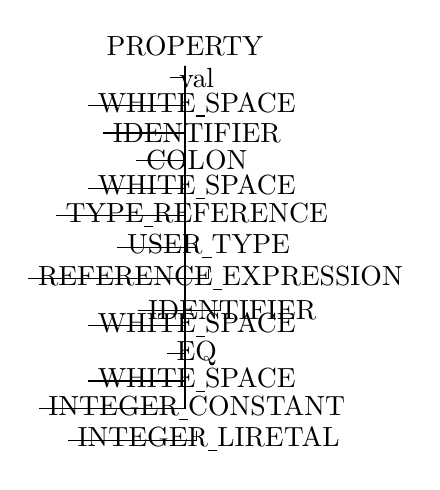
\begin{tikzpicture}[%
  grow via three points={one child at (0.3,-0.8) and
  two children at (0.3,-0.8) and (0.3,-1.5)},
  scale=0.5,
  edge from parent path={(\tikzparentnode.south) |- (\tikzchildnode.west)}]

  \node {PROPERTY}
    child { node {val}}
    child {node {WHITE\underline{ }SPACE}}
    child {node {IDENTIFIER}}
    child {node {COLON}}
    child {node {WHITE\underline{ }SPACE}}
    child {node {TYPE\underline{ }REFERENCE}
    	child {node {USER\underline{ }TYPE}
		child {node {REFERENCE\underline{ }EXPRESSION}
			child {node {IDENTIFIER}}
		}
	}
    }
    child [missing] {}
    child [missing] {}
    child [missing] {}
    child {node {WHITE\underline{ }SPACE}}
    child {node {EQ}}
    child {node {WHITE\underline{ }SPACE}}
    child {node {INTEGER\underline{ }CONSTANT}
    	child {node {INTEGER\underline{ }LIRETAL}}
    };
\end{tikzpicture}
\\

As you can see in the example, we pass the text of the source code, that we want to transform, to the method.  What's going on inside this method? First of all, special system properties (used by Kotlin parser) are set (for example: set "idea.io.use.nio2" to true). If the text of the code contains high-level keywords like \texttt{import} or \texttt{package}, then the method builds a tree with a root node of the FILE type, otherwise it tries with a different root type. In both cases, at the end, if the tree contains a node with type \texttt{ERROR\underline{ }ELEMENT}, it means that some of the code and the method was unable to build the tree and, therefore, throws an exception.\\
This helps us to implement such complex inspections like the detection of commented code (and distinguish real comments from commented code blocks), helps easily fix the code without manually building sub-trees in visitors.\\

\subsection{Suppress annotation}
\par
What if the user wants one of the diKTat Inspections not to check a particular piece of code? The \textsl{SUPPRESS} annotation will help us with it. This annotation can be used to ignore a certain Inspection in a certain code block. For instance, if we run this code:

\begin{lstlisting}[caption={Function with incorrect name.}, label={lst:example1}, language=Kotlin]
/**
 * This is example
 */

package com.saveourtool.diktat

/**
 * Simple class
 */
class User(private val name: String, private val age: Int) {
	/**
	 * Function with incorrect name
	 *
	 * @return is username longer than age
	 */
	fun IsInCoRrEcTnAMe() = name.length > age
}

\end{lstlisting}

Diktat will raise the warning:
$$
\texttt{ \small{ $\big[$FUNCTION\underline{ }NAME\underline{ }INCORRECT\underline{ }CASE$\big]$  function/method name should be in lowerCamelCase}}
$$

But if there is a \texttt{@Suppress} before this method, then there will be no warnings during the run:
\begin{lstlisting}[caption={Function with incorrect name, but with suppressed Inspection.}, label={lst:example1}, language=Kotlin]
/**
 * This is example
 */

package com.saveourtool.diktat

/**
 * Simple class
 */
@Suppress("FUNCTION_NAME_INCORRECT_CASE")
class User(private val name: String, private val age: Int) {
	/**
	 * Function with incorrect name
	 *
	 * @return is username longer than age
	 */
	fun IsInCoRrEcTnAMe() = name.length > age
}

\end{lstlisting}

The example shows that the method has a suppress annotation. Therefore, the \texttt{FUNCTION\underline{ }NAME\underline{ }INCORRECT\underline{ }CASE} rule will be ignored on this method and there will be no error. The search method for a given annotation goes up recursively to the root element of type \texttt{FILE}, looking for the annotation. This means that \texttt{@Suppress} can be placed not only in front of knowingly incorrect code, but also at the upper levels of the abstract syntax tree. In our example, the annotation is not in front of the method, but in front of the class and it still works. Also, you can put several annotations:
\begin{lstlisting}[caption={Several suppression annotations}, label={lst:example1}, language=Kotlin]
@set:[Suppress("WRONG_DECLARATION_ORDER") Suppress("IDENTIFIER_LENGTH")]
\end{lstlisting}

\subsection{WEB}
It worth mentioning that there is a web version of diKTat. This is a handy tool that can be used quickly without any installations, and it is very simple. The link can be found in or you can find it in "\nameref{sec:download}" chapter or in ktlint project as reference.\footnote{\url{https://github.com/pinterest/ktlint\#online-demo}}
\begin{figure}[H]
  \centering
  \includegraphics[scale=0.3]{pictures/web-example.png}
  \caption{Diktat-web online demo}
\end{figure}

\subsection{Options validation}
As it has been mention earlier, diktat has a highly customizable configuration file, but manually editing it is error-prone, for example, name of the rule can be incorrect due to a typo. Diktat will validate configuration file on startup and suggest the closest name based on \textsl{Levenshtein} method.

\subsection{Self checks}
Diktat fully supports self checking of it's own code using both release and snapshot (master) versions. Diktat uses it's self to validate the code inside during it's CI/CD process.


\section{How to use diKTat}
\label{sec:download}
\subsection{CLI-application}
\par You can run diKTat as a CLI-application by installing it first. You can find detailed instructions on how to install and run on different OS on github (\url{https://github.com/cqfn/diKTat/blob/master/README.md#run-as-cli-application}). After the run, errors will be found and displayed. Each error consists of a rule name, a description of the rule so that the user can understands the error, the line and column number where the error was found.\\
\subsection{Plugins}
\par Alternatively, you can add a diktat maven or gradle plugin directly to the project: detailed instructions for maven can be found here - \url{https://github.com/cqfn/diKTat/blob/master/README.md#run-with-maven}and for gralde - \url{https://github.com/cqfn/diKTat/blob/master/README.md#run-with-gradle-plugin}.\\
\subsection{Configuration file}
As described above, diKTat has a configuration file. Note that you should place the \textsl{diktat-analysis.yml} file containing the diktat configuration in the parent directory of your project when running as a CLI application. Diktat-maven-plugin and diktat-gradle-plugin have a separate option for configuration file path.
\subsection{WEB}
\par Of course, the easiest way to use it without any downloads or installations is the web version of the app. You can try it by following the link \url{https://ktlint-demo.herokuapp.com/demo}. Web app supports both checking and fixing, using either ktlint or diktat ruleset. For diktat you can also upload a custom configuration file.


\section{Conclusion \& Future Work}
\label{sec:conclusion}
\par DiKTat is a static code analyzer that finds and fixes code style inconsistencies. DiKTat is configurable, easy-to-use and it implements CI/CD pipelines, which distinguishes it from analogues. We offer many convenient ways to use diktat in projects, so you can use it as Maven/Gradle plugin, CLI tool, Web or github actions(???). It supports more than 100 rules, where each of them has clear explanation and can be configured by user.
\par When the development of diKTat will finish, we are going to support rules, update frameworks and track latest kotlin language releases to keep diKTat relevant.

\newpage
\nocite{*}
\bibliographystyle{ieeetr}
\bibliography{references.bib}

\newpage
\section{Appendix}
\label{sec:appendix}
4-6 sentences. 

\end{CJK*}
\end{document}
